\label{casestudy-proof-chapter}
%\section{Security Verification of mCertiKOS}
%\label{casestudy-proof}

To prove end-to-end security of mCertiKOS, we must apply 
Theorem~\ref{end-to-end} of Chapter~\ref{methodology-chapter}, using 
the simulation from TSysCall-local to MBoot, the high-level observation 
function described in Chapter~\ref{casestudy-def-chapter}, and a low-level
observation function that simply projects the output buffer.
To apply the theorem, the following facts must be established:
\begin{enumerate}
\item MBoot is deterministic.
\item MBoot is behavioral for any principal (Definition~\ref{behavioral-state}
of Chapter~\ref{methodology-chapter}).
\item The simulation from TSysCall-local to MBoot preserves
indistinguishability.
\item TSysCall-local satisfies the high-level security
property (Definition~\ref{high-level-security} of Chapter~\ref{methodology-chapter}).
\end{enumerate}
Determinism of the MBoot machine is already proved in mCertiKOS
(in fact, all layers are deterministic).
Behaviorality of MBoot is easily established by defining 
a partial order over output buffers based on list prefix,
and showing that every step of MBoot either leaves the
buffer untouched or appends to the end of the buffer.
To prove that the simulation preserves indistinguishability,
we first prove that simulation between consecutive layers in
mCertiKOS always preserves the output buffer. 
Property~3 of Definition~\ref{gensimdef} then directly follows,
using an observation translation function $\obsrel{R}$
which simply projects the output buffer.

The primary task of the proof effort is, unsurprisingly, 
establishing the high-level unwinding condition over the
TSysCall-local semantics. The proof is done by showing
that each non-yield primitive of the TSysCall layer preserves 
indistinguishability. The yield primitive requires
special treatment since the TSysCall-local semantics treats
it differently; this will be discussed later in this section.

\begin{figure}
\centering{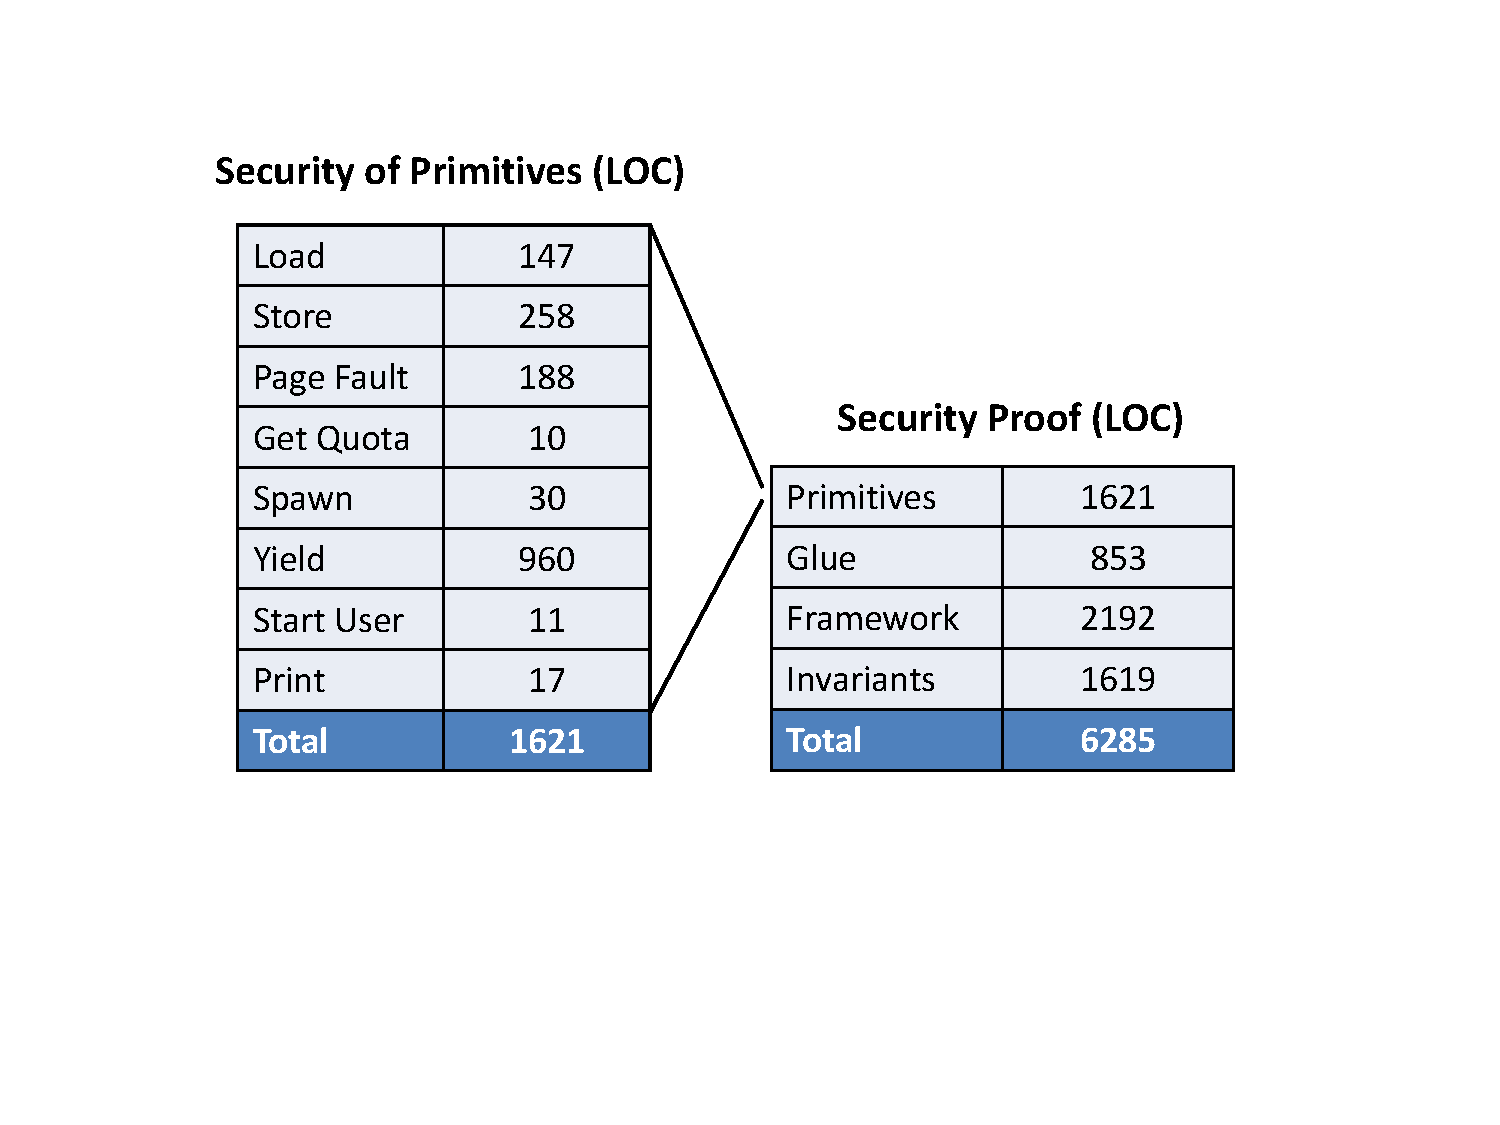
\includegraphics[scale=0.4]{pldi/figure/secure-loc.pdf}}
\caption{\small{Approximate Coq LOC of proof effort.}}
%\vspace*{-1.5ex}
\label{secure-loc}
\end{figure}

Figure~\ref{secure-loc} gives the number of lines of Coq definitions
and proof scripts required for the proof effort. 
The entire effort is broken down into security proofs for
primitives, glue code to interface the primitive
proofs with the LAsm$(L)$ semantics, definitions and proofs
of the framework described in Chapter~\ref{methodology-chapter}, and
proofs of new state invariants that needed to be established.
We will now discuss the most interesting aspects and difficulties 
of the TSysCall-local security proof.

\section{Conducting the TSysCall-local Security Proof}

%\vspace*{-1ex}
\paragraph{State Invariants}
%Some of the following descriptions of security proofs for
%primitives will refer to state invariants.
While mCertiKOS already verifies a number of useful state 
invariants, some new ones are needed for our security proofs.
%These invariants make up the 
%state predicate $I$ mentioned in the end-to-end security 
%theorem of Section~\ref{methodology}.
The most important new invariants established over 
TSysCall-local execution are:
\begin{enumerate}
\item In all saved register contexts, the instruction pointer 
register points to the entry of the 
\ttt{start\_user} primitive.
\item No page is mapped more than once in the page tables.
\item A user process is always either in user mode, or is in kernel mode 
and the instruction pointer register points to the entry of the \ttt{start\_user} 
primitive (meaning that the first part of yield was just executed,
and user mode will be restored in one step).
\item The sum of the available quotas (max quota minus usage) of all
spawned processes is less than or equal to the number of unallocated
pages in the heap (implying that page allocation will always be
successful if the process has quota available).
\end{enumerate}
\cut{
Additionally, for a given observer principal $p$, we assume the
invariant that process $p$ has been spawned. Anything occurring
before the spawning of $p$ is considered part of the 
initialization/configuration phase; we are not interested in 
reasoning about the security of process $p$ before the process
even exists in the system.}

%\vspace*{-1ex}
\paragraph{Security of Load/Store Primitives}
The main task for proving security of the $100$+ assembly commands
of LAsm(TSys\-Call) is to show that the TSysCall layer's load/store 
primitives preserve indistinguishability. This requires showing
that equality of virtual address spaces is preserved. Reasoning 
about virtual address spaces can get quite hairy since we always
have to consider walking through the page tables, with the 
possibility of faulting at either of the two levels.

To better understand the intricacies of this proof, consider the
following situation. Suppose we have two states $\sigma_1$ and
$\sigma_2$ with equal mappings of virtual addresses to option values
(where no value indicates a page fault). Suppose we are writing
to some virtual address $v$ in two executions on these states.
Consider what happens if there exists some other virtual address
$v'$ such that $v$ and $v'$ map to the same physical page
in the first execution, but map to different physical pages in
the second. It is still possible for $\sigma_1$ and $\sigma_2$
to have identical views of their virtual address space, as long
as the two different physical pages in the second execution
contain the same values everywhere. However, writing to $v$
will change the observable view of $v'$ in the first execution,
but not in the second. Hence, in this situation, it is possible
for the store primitive to break indistinguishability.

We encountered this exact counterexample while attempting to
prove security, and we resolved the problem by establishing
the second state invariant mentioned above. The invariant
guarantees that the virtual addresses $v$ and $v'$ will never 
be able to map to the same physical page, thus ruling
out the counterexample.

%%%%%%%%%%%%%%%%%%%%%%%%%%%%%%%%%%%%%%%%%%%%%%%%%%%%%%%%%%%%%%%%
\begin{figure}[t]
\begin{center}
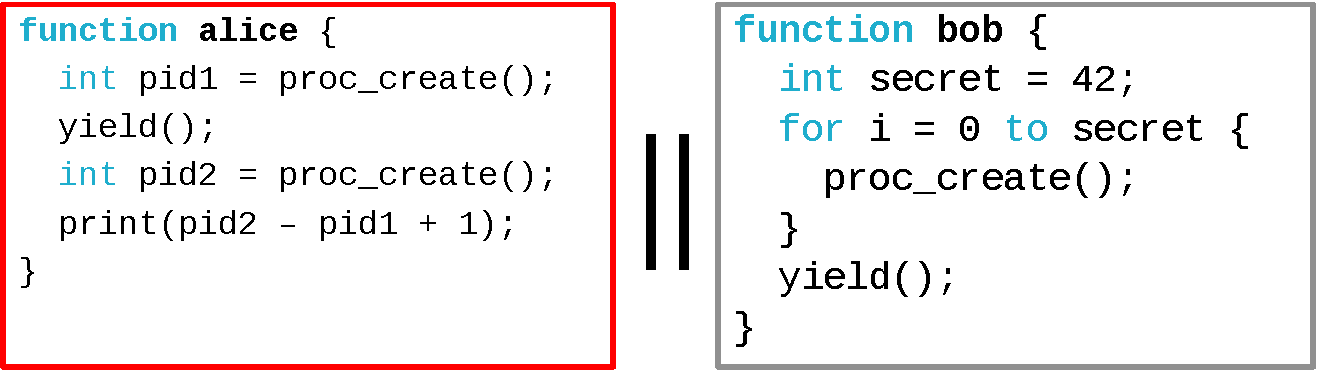
\includegraphics[scale=0.55]{pldi/figure/spawnleak}
\caption{\small Using child process IDs to as a side channel.}
\label{fig:proccreate-leak}
%\vspace*{-20pt}
\end{center}
\end{figure}
%%%%%%%%%%%%%%%%%%%%%%%%%%%%%%%%%%%%%%%%%%%%%%%%%%%%%%%%%%%%%%%%

%\vspace*{-1ex}
\paragraph{Security of Process Spawning}
During our verification effort, we discovered that the \ttt{proc\_create}
primitive had a major security flaw. Figure~\ref{fig:proccreate-leak} 
shows two user programs that exploit \ttt{proc\_create} as
a side channel for communication. When the insecure version of 
mCertiKOS creates a new child process, it chooses the lowest process 
ID not currently in use, and returns the ID to the user. 
\begin{comment}
\begin{alltt}
Alice:                       Bob:
  x = proc\_create();          yield(); 
  yield();                     for (i = 0; i < z; i++)
  y = proc\_create();            proc\_create();
  z = y - x - 1;               yield();
\end{alltt}
\end{comment}
In the figure, Alice spawns a child process, stores its 
ID into variable $x$, and then yields to Bob. Bob 
spawns a number of children equal to some secret value,
and then yields back to Alice. Finally, Alices spawns
another child, stores its ID into $y$, and observes the
value $y-x-1$. This observed value is exactly Bob's
secret!

To close this side channel, we had to revamp the way child
process IDs are chosen in mCertiKOS-secure. The new ID system 
works as follows. We define a global parameter $m$ limiting
the number of children any process is allowed to spawn.
Suppose a process with ID $i$ and $c$ children ($c < m$)
spawns a new child. Then the child's ID will always be
$i*m + c + 1$. This formula guarantees that different
processes can never interfere with each other via child
ID: if $i \neq j$, then the set of possible child IDs for
process $i$ is completely disjoint from the set of
possible child IDs for process $j$. It is easy to see how
this scheme closes the leak of Figure~\ref{fig:proccreate-leak}.
$x$ will always the contain the ID of Alice's first
child, while $y$ will contain the ID of Alice's second
child; these two values are determined solely by Alice's
own ID, so Bob is no longer capable of influencing them.

%\vspace*{-1ex}
\paragraph{Security of Page Fault}
\begin{comment}
There are two different interesting aspects of page-fault
security. The first is that it is a perfect example of 
a primitive whose implementation does not preserve
indistinguishability with each individual step. 
When a page fault occurs, 
either one or two new pages must be allocated from the global 
heap. Because all user processes use the same global heap for 
allocation, and mCertiKOS always allocates the first available
page, the physical address of an allocated page can potentially
leak information between processes. The page fault handler, however,
must make use of the physical address of a newly-allocated page
when inserting a new virtual address mapping into the page
table. Therefore, at some point during the actual (non-atomic)
execution of the page fault handler, an observable register contains
the insecure physical page address. Since we prove that the
primitive's atomic specification is secure, however, we know that
the insecure value must be overwritten by the time the
primitive finishes executing.
\end{comment}
Since page faults dynamically allocate new pages, security
of page faulting requires some reasoning about the resource quota 
implemented by containers (recall the container discussion in 
Chapter~\ref{casestudy-def-chapter}). More specifically, notice
that the global allocation table \ttt{AT} must be unobservable to
user processes since all processes can affect it via page allocation.
This means that the page fault handler may successfully allocate a page 
in one execution, but fail to allocate a page in an execution from
an indistinguishable state due to there being no pages available. 
Clearly, the observable result of the primitive will be different 
for these two executions. To deal with this difficulty, we relate available 
heap pages to available quota by applying the fourth state invariant 
mentioned above. Recall that the invariant guarantees that the sum 
of the available quotas of all spawned processes is always less than 
or equal to the number of available heap pages. Therefore, if an 
execution ever fails to allocate a page because no available page 
exists, the available quota of \emph{all} spawned processes must be 
zero. Since the available quota is observable, we see that allocation 
requests will be denied in both executions from indistinguishable
states. Therefore, we actually \emph{can} end up in
a situation where one execution has pages available for allocation 
while the other does not;
in both executions, however, the available quota will be zero, and
so the page allocator will deny the request for allocation.

%\vspace*{-1ex}
\begin{figure}
\centering{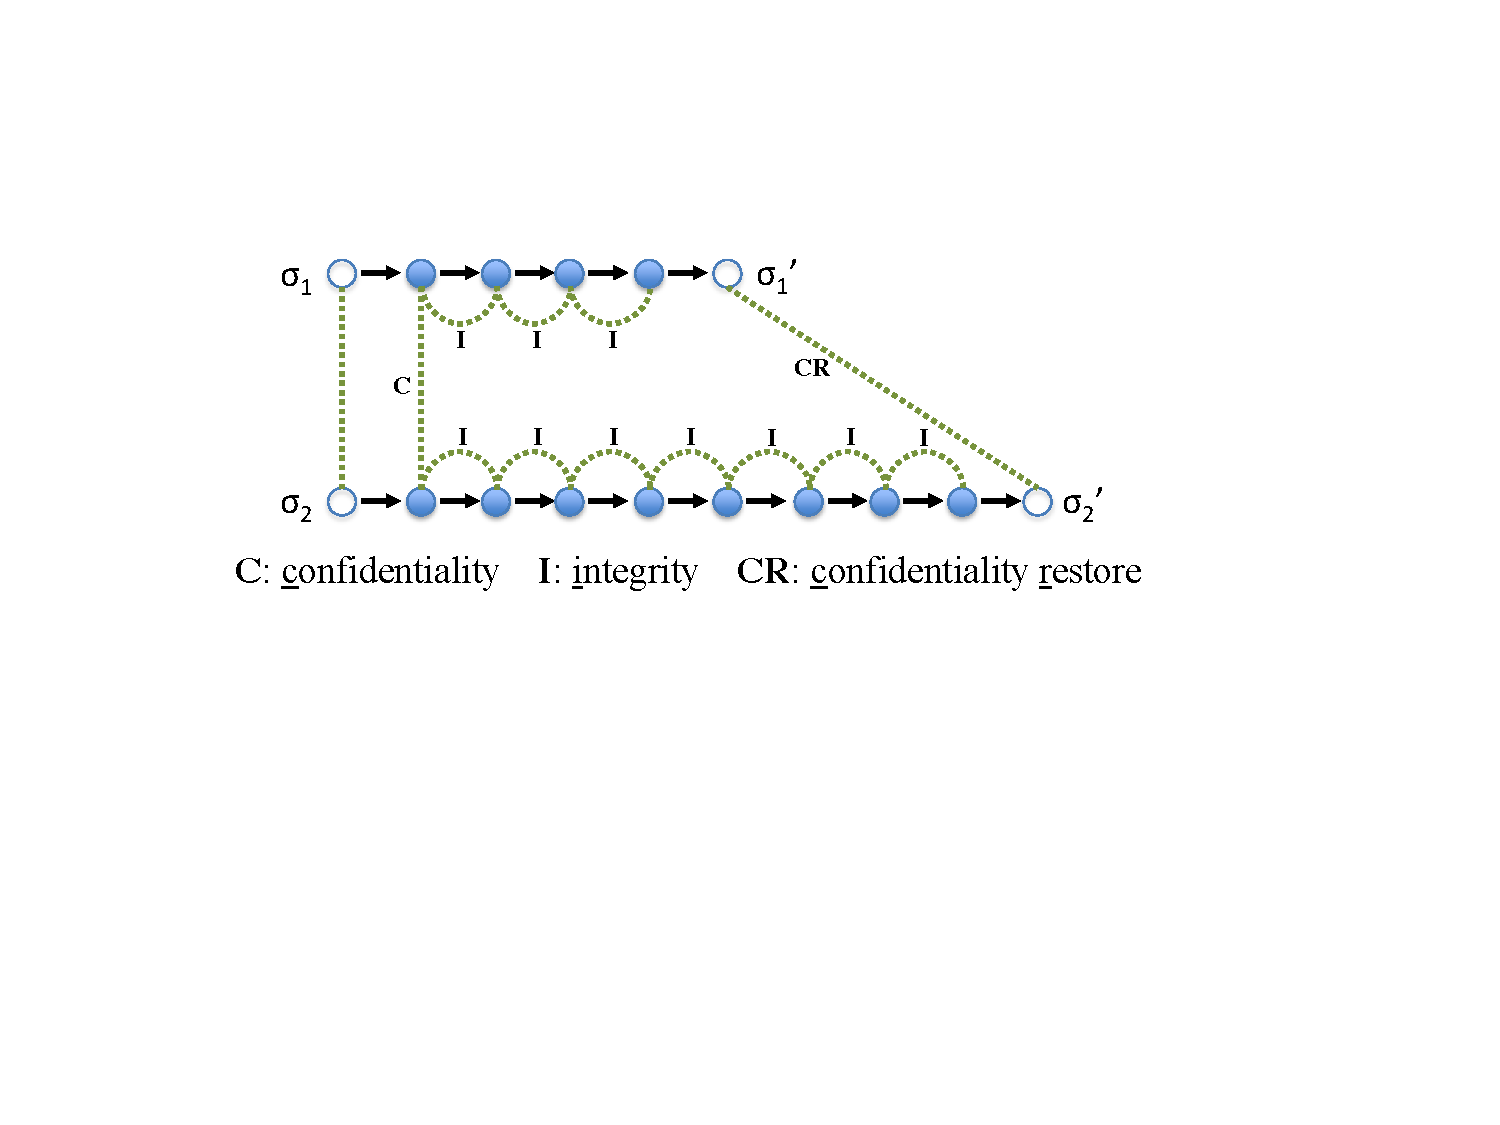
\includegraphics[scale=0.53]{pldi/figure/lemmas.pdf}}
\caption{\small Applying the three lemmas to prove the security
property of TSysCall-local yielding.}
%\vspace*{-3ex}
\label{bigstep-sec}
\end{figure}
\paragraph{Security of Yield}
Yielding is by far the most complex primitive to prove secure,
as the proof requires reasoning about the relationship between
the TSysCall semantics and TSysCall-local semantics. Consider
Figure~\ref{bigstep-sec}, where active states $\sigma_1$ and
$\sigma_2$ are indistinguishable, and they both call yield. 
The TSysCall-local semantics takes a big step over the executions 
of all non-observer processes;
these big steps are unfolded in Figure~\ref{bigstep-sec},
so the solid arrows are all of the individual steps of the 
TSysCall semantics. We must establish that a big-step yield
of the TSysCall-local machine preserves indistinguishability, 
meaning that states $\sigma_1'$ and $\sigma_2'$ in 
Figure~\ref{bigstep-sec} must be proved indistinguishable.
We divide this proof into three separate lemmas, proved over 
the TSysCall semantics:
\begin{itemize} \itemsep 0pt
\item \emph{Confidentiality}~--- If two indistinguishable
active states take a step to two inactive states, then those
inactive states are indistinguishable.
\item \emph{Integrity}~--- If an inactive state takes a step
to another inactive state, then those states are 
indistinguishable.
\item \emph{Confidentiality Restore}~--- If two indistinguishable
inactive states take a step to two active states, then those
active states are indistinguishable.
\end{itemize}
These lemmas are chained together as pictured in 
Figure~\ref{bigstep-sec}. The dashed lines indicate
indistinguishability. Thus the confidentiality lemma
establishes indistinguishability of the initial inactive
states after yielding, the integrity lemma establishes
indistinguishability of the inactive states immediately
preceding a yield back to the observer process, and the
confidentiality restore lemma establishes indistinguishability
of the active states after yielding back to the observer process.
%Therefore, these three lemmas together demonstrate that
%a big-step yield in the TSysCall-local machine preserves
%indistinguishability.

\ifextended
In the mCertiKOS proof, we actually generalize the confidentiality
lemma to apply to other primitives besides yield.
\begin{itemize}
\item \emph{Generalized Confidentiality}~--- Two indistinguishable
active states always take a step to indistinguishable states.
\end{itemize}
We frame all of the high-level security proofs for the other
primitives as instances of this confidentiality lemma. This
means that we derive high-level security of the entire TSysCall-local
machine by proving this generalized confidentiality lemma along with 
integrity and confidentiality restore.
\else\fi

Note that while the confidentiality and confidentiality restore
lemmas apply specifically to the yield primitive (since it is
the only primitive that can change active status), the
integrity lemma applies to all primitives.
Thus, like the security unwinding condition, integrity is proved 
for each of the TSysCall primitives. The integrity proofs are 
simpler since the integrity property only requires 
reasoning about a single execution, whereas security requires 
comparing two.

The confidentiality restore lemma only applies to the situation
where two executions are both yielding back 
to the observer process. The primary obligation
of the proof is to show that if the saved register contexts of two
states $\sigma_1$ and $\sigma_2$ are equal, then the actual registers
of the resulting states $\sigma_1'$ and $\sigma_2'$ are equal.
There is one interesting detail related to this proof:
a context switch in mCertiKOS does not save \emph{every} machine
register\maybecut{, but instead only saves those registers that are relevant
to the local execution of a process (e.g., EAX, ESP, etc.).}
In particular, the CR2 register, which the page fault handler
primitive depends on, is not saved. This means that, immediately
after a context switch from some process $i$ to some other process 
$j$, the CR2 register could contain a virtual address that is private 
to~$i$. How can we then guarantee that $j$ is not influenced by this
value? Indeed, if process $j$ is able to immediately call the page 
fault handler without first triggering a page fault, then it may very 
well learn some information about process $i$. We resolve this potential
leak by making a very minor change to mCertiKOS: we add a line of
assembly code to the implementation of context switch that clears
the CR2 register to zero.

\ifextended
\paragraph{Security of Other Primitives}

We do not need to reason about security of \ttt{proc\_init}
since we assume that initialization occurs appropriately,
and no process is ever allowed to call the primitive again after 
initialization finishes. None of the primitives \ttt{get\_quota}, 
\ttt{start\_user}, or \ttt{print} brought up any difficulties
for security verification.
\else\fi

\section{End-to-End Process Isolation}
\label{casestudy-isolation}

We conclude this chapter by taking a step back and revisiting the
top-level end-to-end security theorem. The final 
statement is the conclusion of Theorem~\ref{end-to-end}, which
is low-level security of the MBoot machine for all states
related by $\phi(M,p,I,R)$. In other words, the theorem says
that if we consider any MBoot state $s_1$ related to a
properly-initialized TSysCall state $\sigma_1$, and
we consider related modified states $s_2$ and $\sigma_2$
with $\sigma_2$ initialized and $\observe{p}{\sigma_1} = \observe{p}{\sigma_2}$, 
then the whole-execution behaviors of MBoot on $s_1$ and $s_2$
are identical. Notice that this statement requires a solid 
understanding of the particular mCertiKOS observation function. 
While it may feel intuitively clear that the observation function
defined in Section~\ref{ssec:security-overview} is reasonable,
how can we be certain? Poorly-defined observation functions are
certainly possible; for example, if we define an identity observation
function where all principals observe all program state, then 
the unwinding condition degenerates
into a simple statement of determinism. Thus applying our methodology
with such an observation function would not actually give us a result 
that is related to security.

In general, we consider the observation function definition to
be a trusted part of the methodology, in the same way that high-level
specifications must be trusted to actually specify our intuitive
desires for the software's behavior. However, depending on the
context, we may be able to do better than this. While we have not
yet completed a formal Coq development, we hope to prove a higher-level
end-to-end security theorem in mCertiKOS that truly guarantees 
user-process isolation by being completely independent from the choice 
of observation function. Our vision for how this would work involves
the following two steps:
\begin{enumerate}
\item Define a new state predicate $\spawned{p}$, saying that process
$p$ was \emph{just spawned} by the kernel. Prove that this predicate
is stronger than the initialization predicate $I$ 
(i.e., $\forall p \such \spawned{p} \Rightarrow I$).
\item Prove that \emph{all} states satisfying $\spawned{p}$ are
indistinguishable from one another according to $p$
(i.e., $\forall \sigma_1, \sigma_2 \in \spawned{p} \such 
\observe{p}{\sigma_1} = \observe{p}{\sigma_2}$). We imagine that
such a property should be provable since all of $p$'s data should
be in a deterministic initial state (e.g., all zeros) immediately 
after $p$ is spawned.
\end{enumerate}
Assuming we can successfully implement these steps, the end-to-end
security guarantee can clearly be reformulated as follows: if we consider
some MBoot state $s_1$ that is related to a TSysCall state $\sigma_1$
which occurs immediately after $p$ is spawned (i.e., $\sigma_1 \in \spawned{p}$), 
along with related modified states $s_2$ and $\sigma_2$ (with
$\sigma_2 \in \spawned{p}$), then the 
whole-execution behaviors of MBoot on $s_1$ and $s_2$ are identical.
With this theorem formulation, we no longer need to understand and
trust the choice of observation function. While we still have some
details to work out, we are hopeful that such a theorem can be 
established in the near future.


